\section{Isomorfismos}

\subsection{}

{\nologo 
\begin{frame}\frametitle{Transformaciones lineales uno a uno}

\vspace{-3mm}
\begin{block}{\textbf{Definición 1 (uno a uno) }}
	\justifying
	Una transformación lineal $T:V\to W$ se dice que es \textbf{\textit{inyectiva}} o \textbf{\textit{uno a uno}} (1--1) si
	para cada par de vectores $\mathbf{u}$ y $\mathbf{v}$ en $V$,
	\[
		\mathbf{u}\neq \mathbf{v} \quad \text{implica} \quad T(\mathbf{u})\neq T(\mathbf{v}).
	\]
\end{block}

\vspace{-1mm}
\begin{alertblock}{\textbf{Observación 1}}
	\begin{figure}	
		\begin{subfigure}[b]{0.3\textwidth}
			\centering
			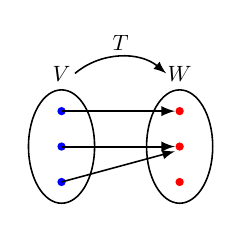
\begin{tikzpicture}[thick,scale=0.3, every node/.style={scale=0.8}]%[scale=.5]
			\draw[line width=0.2mm] (0,0) ellipse (1.4 and 2.4);
			\node[above] at (0,2.4) {$V$}; \node[above] at (5,2.4) {$W$};
			\fill[color=blue] (0,1.5) circle[radius=5pt]; %\node (a) at (0,1.5) {$1$}; 
			\fill[color=blue] (0,0) circle[radius=5pt];	 %\node (b) at (0,0) {$2$};
			\fill[color=blue] (0,-1.5) circle[radius=5pt]; %\node (c) at (0,-1.5) {$3$};
			\draw[line width=0.2mm] (5,0) ellipse (1.4 and 2.4);
			\fill[color=red] (5,1.5) circle[radius=5pt]; %\node (a1) at (5,1.5) {$a$}; 
			\fill[color=red] (5,0) circle[radius=5pt]; %\node (b1) at (5,0) {$b$};		
			\fill[color=red] (5,-1.5) circle[radius=5pt]; %\node (c1) at (5,-1.5) {$c$};
			\draw[line width=0.25mm,-latex] (0,1.5) -- (4.8,1.5); %\draw[line width=0.2mm,-latex] (a)--(a1); 
			\draw[line width=0.25mm,-latex] (0,0) -- (4.8,0); %\draw[line width=0.2mm,-latex] (b)--(b1); 
			\draw[line width=0.2mm,-latex] (0,-1.5) -- (4.8,-0.2); %\draw[thick,-latex] (c)--(b1);
			\draw[line width=0.2mm,latex-] (2.5,0.8) +(50:3cm) arc (50:130:3cm);
			\node at (2.5,4.4) {$T$};
			\end{tikzpicture}
			\caption{$T$ \textbf{no} es uno a uno}
		\end{subfigure}
		\hspace{1cm}
		\begin{subfigure}[b]{0.3\textwidth}
			\centering
			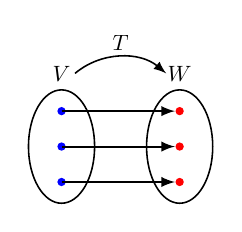
\begin{tikzpicture}[thick,scale=0.3, every node/.style={scale=0.8}]%[scale=.5]
			\draw[line width=0.2mm] (0,0) ellipse (1.4 and 2.4);
			\node[above] at (0,2.4) {$V$}; \node[above] at (5,2.4) {$W$};
			\fill[color=blue] (0,1.5) circle[radius=5pt]; %\node (a) at (0,1.5) {$1$}; 
			\fill[color=blue] (0,0) circle[radius=5pt];	 %\node (b) at (0,0) {$2$};
			\fill[color=blue] (0,-1.5) circle[radius=5pt]; %\node (c) at (0,-1.5) {$3$};
			\draw[line width=0.2mm] (5,0) ellipse (1.4 and 2.4);
			\fill[color=red] (5,1.5) circle[radius=5pt]; %\node (a1) at (5,1.5) {$a$}; 
			\fill[color=red] (5,0) circle[radius=5pt]; %\node (b1) at (5,0) {$b$};		
			\fill[color=red] (5,-1.5) circle[radius=5pt]; %\node (c1) at (5,-1.5) {$c$};
			\draw[line width=0.25mm,-latex] (0,1.5) -- (4.8,1.5); %\draw[line width=0.2mm,-latex] (a)--(a1); 
			\draw[line width=0.25mm,-latex] (0,0) -- (4.8,0); %\draw[line width=0.2mm,-latex] (b)--(b1); 
			\draw[line width=0.25mm,-latex] (0,-1.5) -- (4.8,-1.5); %\draw[thick,-latex] (c)--(b1);
			\draw[line width=0.2mm,latex-] (2.5,0.8) +(50:3cm) arc (50:130:3cm);
			\node at (2.5,4.4) {$T$};
			\end{tikzpicture}
			\caption{$T$ es uno a uno}
		\end{subfigure}
	\end{figure}
\end{alertblock}

\vspace{-1mm}
\begin{prop}{\textbf{Propiedad 1}}
	\justifying
	$T:V\to W$ es \textbf{\textit{uno a uno}} si 
	
	\vspace{-2mm}
	\[
	T(\mathbf{u}) = T(\mathbf{v}) \quad \text{implica} \quad \mathbf{u} = \mathbf{v}.
	\]
\end{prop}	

\end{frame}
}

% ---------------------------------------------------------------------------------------------------

\subsection{}

{\nologo 
\begin{frame}\frametitle{Transformaciones lineales uno a uno}

\begin{block}{\textbf{Definición 1 (uno a uno) }}
	\justifying
	Una transformación lineal $T:V\to W$ se dice que es \textbf{\textit{inyectiva}} o \textbf{\textit{uno a uno}} (1--1) si
	para cada par de vectores $\mathbf{u}$ y $\mathbf{v}$ en $V$,
	\[
	\mathbf{u}\neq \mathbf{v} \quad \text{implica} \quad T(\mathbf{u})\neq T(\mathbf{v}).
	\]
\end{block}

\begin{prop}{\textbf{Propiedad 1}}
	\justifying
	$T:V\to W$ es \textbf{\textit{uno a uno}} si 
	
	\vspace{-2mm}
	\[
	T(\mathbf{u}) = T(\mathbf{v}) \quad \text{implica} \quad \mathbf{u} = \mathbf{v}.
	\]
\end{prop}	

\begin{prop}{\textbf{Propiedad 2}}
	\justifying
	Sea $T:V\to W$ transformación lineal. Entonces $T$ es uno a uno si y sólo si 
	\[
	\text{nu}\,T=\{\mathbf{0}\}.
	\]
\end{prop}	

\end{frame}
}

% ---------------------------------------------------------------------------------------------------

\subsection{}

\begin{frame}\frametitle{Transformaciones lineales uno a uno y no uno a uno}
	
	\begin{prop}{\textbf{Propiedad 2}}
		\justifying
		Sea $T:V\to W$ transformación lineal. Entonces $T$ es uno a uno si y sólo si 
		\[
		\text{nu}\,T=\{\mathbf{0}\}.
		\]
	\end{prop}	
	
	\begin{ej}{\textbf{Ejemplo 1}}
		\justifying
		Considere la transformación lineal  $T:M_{mn}\to M_{nm}$ definida por 
		\[
		T(A) = A^T.
		\]
		Demuestre que $T$ es \textit{uno a uno}.
		
	\end{ej}
	\textit{Solución.}
	
\end{frame}

% ---------------------------------------------------------------------------------------------------

\subsection{}

{\nologo 
\begin{frame}\frametitle{Transformaciones lineales uno a uno y no uno a uno}

\begin{prop}{\textbf{Propiedad 2}}
	\justifying
	Sea $T:V\to W$ transformación lineal. Entonces $T$ es uno a uno si y sólo si 
	\[
	\text{nu}\,T=\{\mathbf{0}\}.
	\]
\end{prop}	

\begin{ej}{\textbf{Ejemplo 2}}
	\justifying
	Considere la transformación lineal cero $T:\r^2\to \r^2$ definida por
	\[
	T(\mathbf{v}) = \mathbf{0}, \quad \text{ para todo } \mathbf{v} \text{ en } \r^2.
	\]
	Demuestre que $T$ no es \textit{uno a uno}.
\end{ej}
\textit{Solución.}

\end{frame}
}

% ---------------------------------------------------------------------------------------------------

\subsection{}

{\nologo 
\begin{frame}\frametitle{Transformaciones lineales sobre}

\vspace{-3mm}
\begin{block}{\textbf{Definición 2 (sobre) }}
	\justifying
	Una transformación lineal $T:V\to W$ se dice que es \textbf{\textit{sobreyectiva}} o \textbf{\textit{sobre}} si
	todo vector en $W$ tiene una preimagen en $V$. Es decir, para todo $\mathbf{w}$ en $W$, existe al menos un
	 $\mathbf{v}$ en $V$ tal que $T(\mathbf{v})=\mathbf{w}$.
\end{block}

\vspace{-1mm}
\begin{alertblock}{\textbf{Observación 2}}
	\begin{figure}	
		\begin{subfigure}[b]{0.3\textwidth}
			\centering
			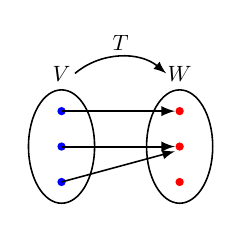
\begin{tikzpicture}[thick,scale=0.3, every node/.style={scale=0.8}]%[scale=.5]
			\draw[line width=0.2mm] (0,0) ellipse (1.4 and 2.4);
			\node[above] at (0,2.4) {$V$}; \node[above] at (5,2.4) {$W$};
			\fill[color=blue] (0,1.5) circle[radius=5pt]; %\node (a) at (0,1.5) {$1$}; 
			\fill[color=blue] (0,0) circle[radius=5pt];	 %\node (b) at (0,0) {$2$};
			\fill[color=blue] (0,-1.5) circle[radius=5pt]; %\node (c) at (0,-1.5) {$3$};
			\draw[line width=0.2mm] (5,0) ellipse (1.4 and 2.4);
			\fill[color=red] (5,1.5) circle[radius=5pt]; %\node (a1) at (5,1.5) {$a$}; 
			\fill[color=red] (5,0) circle[radius=5pt]; %\node (b1) at (5,0) {$b$};		
			\fill[color=red] (5,-1.5) circle[radius=5pt]; %\node (c1) at (5,-1.5) {$c$};
			\draw[line width=0.25mm,-latex] (0,1.5) -- (4.8,1.5); %\draw[line width=0.2mm,-latex] (a)--(a1); 
			\draw[line width=0.25mm,-latex] (0,0) -- (4.8,0); %\draw[line width=0.2mm,-latex] (b)--(b1); 
			\draw[line width=0.2mm,-latex] (0,-1.5) -- (4.8,-0.2); %\draw[thick,-latex] (c)--(b1);
			\draw[line width=0.2mm,latex-] (2.5,0.8) +(50:3cm) arc (50:130:3cm);
			\node at (2.5,4.4) {$T$};
			\end{tikzpicture}
			\caption{$T$ \textbf{no} es sobre}
		\end{subfigure}
		\hspace{1cm}
		\begin{subfigure}[b]{0.3\textwidth}
			\centering
			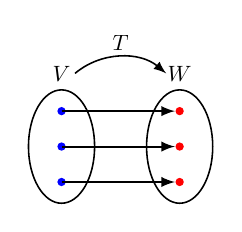
\begin{tikzpicture}[thick,scale=0.3, every node/.style={scale=0.8}]%[scale=.5]
			\draw[line width=0.2mm] (0,0) ellipse (1.4 and 2.4);
			\node[above] at (0,2.4) {$V$}; \node[above] at (5,2.4) {$W$};
			\fill[color=blue] (0,1.5) circle[radius=5pt]; %\node (a) at (0,1.5) {$1$}; 
			\fill[color=blue] (0,0) circle[radius=5pt];	 %\node (b) at (0,0) {$2$};
			\fill[color=blue] (0,-1.5) circle[radius=5pt]; %\node (c) at (0,-1.5) {$3$};
			\draw[line width=0.2mm] (5,0) ellipse (1.4 and 2.4);
			\fill[color=red] (5,1.5) circle[radius=5pt]; %\node (a1) at (5,1.5) {$a$}; 
			\fill[color=red] (5,0) circle[radius=5pt]; %\node (b1) at (5,0) {$b$};		
			\fill[color=red] (5,-1.5) circle[radius=5pt]; %\node (c1) at (5,-1.5) {$c$};
			\draw[line width=0.25mm,-latex] (0,1.5) -- (4.8,1.5); %\draw[line width=0.2mm,-latex] (a)--(a1); 
			\draw[line width=0.25mm,-latex] (0,0) -- (4.8,0); %\draw[line width=0.2mm,-latex] (b)--(b1); 
			\draw[line width=0.25mm,-latex] (0,-1.5) -- (4.8,-1.5); %\draw[thick,-latex] (c)--(b1);
			\draw[line width=0.2mm,latex-] (2.5,0.8) +(50:3cm) arc (50:130:3cm);
			\node at (2.5,4.4) {$T$};
			\end{tikzpicture}
			\caption{$T$ es sobre}
		\end{subfigure}
	\end{figure}
\end{alertblock}

\vspace{-1mm}
\begin{prop}{\textbf{Propiedad 3}}
	\justifying
	$T:V\to W$ es \textbf{\textit{sobre}} si y sólo si
	
	\vspace{-2mm}
	\[
		\text{im}\,T = W.
	\]
\end{prop}	

\end{frame}
}

% ---------------------------------------------------------------------------------------------------

\subsection{}

{\nologo 
\begin{frame}\frametitle{Transformaciones lineales sobre}

\begin{prop}{\textbf{Propiedad 3}}
	\justifying
	$T:V\to W$ es \textbf{\textit{sobre}} si y sólo si
	
	\vspace{-2mm}
	\[
	\text{im}\,T = W.
	\]
\end{prop}	

\begin{prop}{\textbf{Propiedad 4}}
	\justifying
	Sea $T:V\to W$ una transformación lineal y $W$ un espacio vectorial de dimensión finita. Entonces $T$ es \textit{sobre} 
	si y sólo si
	
	\vspace{-2mm}
	\[
		\rho(T) = \dim W.
	\]
\end{prop}	

\begin{prop}{\textbf{Propiedad 5}}
	\justifying
	Sea $T:V\to W$ una transformación lineal, con $V$ y $W$ ambos espacios vectoriales de dimensión $n$. Entonces $T$ es \textit{uno a uno} 
	si y sólo si $T$ es \textit{sobre}.
\end{prop}	

\end{frame}
}

% ---------------------------------------------------------------------------------------------------

\subsection{}

\begin{frame}\frametitle{Transformaciones lineales uno a uno y sobre}

\begin{ej}{\textbf{Ejemplo 3}}
	\justifying
	Para cada una de las matrices $A$ dadas a continuación, encuentre la nulidad y el rango de la transformación lineal 
	$T:\r^n\to \r^m$ definida por $T(\mathbf{x}) = A\mathbf{x}$. 		
	%	\vspace{-1mm}
	\begin{multicols}{4}
		\begin{enumerate}
			\item[\labelname{$a$}] \scalebox{0.82}{$
			\left(
			\begin{array}{@{\hspace{0.3\tabcolsep}}r@{\hspace{1.5\tabcolsep}}r@{\hspace{1.5\tabcolsep}}r@{\hspace{0.3\tabcolsep}}}
			1 & 2 & 0 \\[1mm]
			0 & 1 & 1\\[1mm]
			0 & 0 & 1
			\end{array}
			\right)
			$
			}
			\item[\labelname{$b$}] \scalebox{0.82}{$
			\left(
			\begin{array}{@{\hspace{0.3\tabcolsep}}r@{\hspace{1.5\tabcolsep}}r@{\hspace{0.3\tabcolsep}}}
			1 & 2  \\[1mm]
			0 & 1 \\[1mm]
			0 & 0 
			\end{array}
			\right)
			$
			}
		
			\item[\labelname{$c$}] \scalebox{0.82}{$
			\left(
			\begin{array}{@{\hspace{0.3\tabcolsep}}r@{\hspace{1.5\tabcolsep}}r@{\hspace{1.5\tabcolsep}}r@{\hspace{0.3\tabcolsep}}}
			1 & 2 & 0 \\[1mm]
			0 & 1 & -1
			\end{array}
			\right)
			$
			}	
			\item[\labelname{$d$}] \scalebox{0.82}{$
			\left(
			\begin{array}{@{\hspace{0.3\tabcolsep}}r@{\hspace{1.5\tabcolsep}}r@{\hspace{1.5\tabcolsep}}r@{\hspace{0.3\tabcolsep}}}
			1 & 2 & 0 \\[1mm]
			0 & 1 & 1\\[1mm]
			0 & 0 & 0
			\end{array}
			\right)
			$
			}					
		\end{enumerate}				
	\end{multicols}
	Determine en cada caso si la transformación lineal es \textit{uno a uno} y/o \textit{sobre}.
\end{ej}
\textit{Solución.}

\end{frame}

% ---------------------------------------------------------------------------------------------------

\subsection{}

\begin{frame}\frametitle{Transformaciones lineales uno a uno y sobre}
	
	\begin{prop}{\textbf{Propiedad 6}}
		\justifying
		Sea $V$ y $W$ espacios vectoriales de dimensión finita y $T:V\to W$ una transformación lineal. 
		\begin{enumerate}
			\item[\labelname{$a$}] Si $\dim V > \dim W$, entonces $T$ no es \textit{uno a uno}.
			\item[\labelname{$b$}] Si $\dim V < \dim W$, entonces $T$ no es \textit{sobre}.
		\end{enumerate}
	\end{prop}	
	
	
\end{frame}

% ---------------------------------------------------------------------------------------------------

\subsection{}

\begin{frame}\frametitle{Transformaciones lineales uno a uno y sobre}

\begin{prop}{\textbf{Propiedad 6}}
	\justifying
	Sea $V$ y $W$ espacios vectoriales de dimensión finita y $T:V\to W$ una transformación lineal. 
	\begin{enumerate}
		\item[\labelname{$a$}] Si $\dim V > \dim W$, entonces $T$ no es \textit{uno a uno}.
		\item[\labelname{$b$}] Si $\dim V < \dim W$, entonces $T$ no es \textit{sobre}.
	\end{enumerate}
\end{prop}	

\begin{ej}{\textbf{Ejemplo 4}}
	\justifying
	Determine si la transformación lineal dada a continuación es \textit{uno a uno}.
	\[
		T
		\left(
		\begin{array}{@{\hspace{0.3\tabcolsep}}c@{\hspace{0.3\tabcolsep}}}
		x  \\[1mm]
		y  \\[1mm]
		z
		\end{array}
		\right)
		=
		\left(
		\begin{array}{@{\hspace{0.3\tabcolsep}}r@{\hspace{1.5\tabcolsep}}r@{\hspace{1.5\tabcolsep}}r@{\hspace{0.3\tabcolsep}}}
		1 & 2 & 3 \\[1mm]
		4 & 5 & 6
		\end{array}
		\right)
		\left(
		\begin{array}{@{\hspace{0.3\tabcolsep}}c@{\hspace{0.3\tabcolsep}}}
		x  \\[1mm]
		y  \\[1mm]
		z
		\end{array}
		\right).
	\]
\end{ej}
\textit{Solución.}

\end{frame}

% ---------------------------------------------------------------------------------------------------

\subsection{}

\begin{frame}\frametitle{Transformaciones lineales uno a uno y sobre}

\begin{prop}{\textbf{Propiedad 6}}
	\justifying
	Sea $V$ y $W$ espacios vectoriales de dimensión finita y $T:V\to W$ una transformación lineal. 
	\begin{enumerate}
		\item[\labelname{$a$}] Si $\dim V > \dim W$, entonces $T$ no es \textit{uno a uno}.
		\item[\labelname{$b$}] Si $\dim V < \dim W$, entonces $T$ no es \textit{sobre}.
	\end{enumerate}
\end{prop}	

\begin{ej}{\textbf{Ejemplo 5}}
	\justifying
	Determine si la transformación lineal dada a continuación es \textit{sobre}.
	\[
	T
	\left(
	\begin{array}{@{\hspace{0.3\tabcolsep}}c@{\hspace{0.3\tabcolsep}}}
	x  \\[1mm]
	y  
	\end{array}
	\right)
	=
	\left(
	\begin{array}{@{\hspace{0.3\tabcolsep}}r@{\hspace{1.5\tabcolsep}}r@{\hspace{0.3\tabcolsep}}}
	1 & 2  \\[1mm]
	3 & 4  \\[1mm]
	5 & 6 
	\end{array}
	\right)
	\left(
	\begin{array}{@{\hspace{0.3\tabcolsep}}c@{\hspace{0.3\tabcolsep}}}
	x  \\[1mm]
	y  
	\end{array}
	\right).
	\]
\end{ej}
\textit{Solución.}

\end{frame}

% ---------------------------------------------------------------------------------------------------

\subsection{}

{\nologo 
\begin{frame}\frametitle{Isomorfismos}
	
	\begin{block}{\textbf{Definición 3 (Isomorfismo) }}
		\justifying
		Sea $T:V\to W$ un  transformación lineal. Se dice que $T$ es un \textbf{\textit{isomorfismo}} si
		$T$ es \textit{uno a uno} y \textit{sobre}.
	\end{block}
	
	\begin{block}{\textbf{Definición 4 (Espacios isomorfos) }}
		\justifying
		Sean $V$ y $W$ espacios vectoriales. Se dice que $V$ y $W$ son \textbf{\textit{isomorfos}} si existe una 
		transformación lineal $T:V\to W$ que es \textit{isomorfismo}.
	\end{block}
	
	\begin{alertblock}{\textbf{Observación 3}}
		Sean $V$ y $W$ espacios vectoriales.
		\begin{enumerate}
			\item[\labelname{$a$}] Cuando $V$ y $W$ son isomorfos escribimos $V\cong W$.
			\item[\labelname{$b$}] Los espacios vectoriales isomorfos son ``esencialmente iguales'' en
			el sentido  que tienen la misma dimensión (teorema).
		\end{enumerate}
	\end{alertblock}	
		
\end{frame}
}

% ---------------------------------------------------------------------------------------------------

\subsection{}

\begin{frame}%\frametitle{Isomorfismos}

\begin{block}{\textbf{Definición 3 (Isomorfismo) }}
	\justifying
	Sea $T:V\to W$ un  transformación lineal. Se dice que $T$ es un \textbf{\textit{isomorfismo}} si
	$T$ es \textit{uno a uno} y \textit{sobre}.
\end{block}

\begin{block}{\textbf{Definición 4 (Espacios isomorfos) }}
	\justifying
	Sean $V$ y $W$ espacios vectoriales. Se dice que $V$ y $W$ son \textbf{\textit{isomorfos}} si existe una 
	transformación lineal $T:V\to W$ que es \textit{isomorfismo}.
\end{block}

\begin{ej}{\textbf{Ejemplo 6}}%\justifying
	Demuestre que $T:\r^3\to P_2$ definida por $T(a,b,c)=a+bx+cx^2$ es un isomorfismo.
\end{ej}
\textit{Demostración.}
	
\end{frame}

% ---------------------------------------------------------------------------------------------------

\subsection{}

\begin{frame}\frametitle{Propiedades de los isomorfismos}
	
	\begin{prop}{\textbf{Propiedad 6}}
		\justifying
		Sea $T:\r^n\to \r^n$ una transformación lineal. Las siguientes afirmaciones 
		son equivalentes (si una es verdadera, todas las otras también son verdaderas). 
		\begin{enumerate}[$a$]
			\item $T$ es invertible.			
			\item $T$ es un isomorfismo.
			\item  $A_T$ es invertible y $A_{T^{-1}}= \left(A_T\right)^{-1}$
		\end{enumerate}
	\end{prop}	
	
	
\end{frame}


% ---------------------------------------------------------------------------------------------------

\subsection{}

{\nologo 
\begin{frame}\frametitle{Propiedades de los isomorfismos}
	
	\begin{prop}{\textbf{Propiedad 7}}
		\justifying
		Sea $A$ una matriz $n\times n$. Las siguientes afirmaciones son equivalentes (si una es verdadera, todas
		las otras también son verdaderas). 
		\begin{enumerate}[$a$]\justifying 
			\item $A$ es invertible (no singular).
			\item La única solución al sistema homogéneo $A\mathbf{x} = \mathbf{0}$ es la solución 
			trivial $\mathbf{x}=\mathbf{0}$.
			\item  El sistema $A\mathbf{x} = \mathbf{b}$ tiene solución única para cada vector columna
			$\mathbf{b}$.
			\item $A$ es \textit{equivalente por renglones} a la matriz identidad $I_n$.
			\item $A$ se puede expresar como el producto de matrices elementales.
			\item Las columnas (y renglones) de $A$ son linealmente independientes.
			\item $\det A\neq 0$.
			\item $\nu(A)=0$.
			\item $\rho(A)=n$.
			\item La transformación lineal $T(\mathbf{x})=A\mathbf{x}$ es un isomorfismo.
		\end{enumerate}
	\end{prop}	
	
\end{frame}
}

% ---------------------------------------------------------------------------------------------------

\subsection{}

\begin{frame}\frametitle{Propiedades de los isomorfismos}
	
	\begin{prop}{\textbf{Propiedad 8}}
		\justifying
		Sea $T:V\to W$ un isomorfismo. 
		\begin{enumerate}
			\item[\labelname{$a$}] Si $\mathbf{v}_1, \hdots,\mathbf{v}_n$ generan a $V$, entonces
			$T(\mathbf{v}_1), \hdots,T(\mathbf{v}_n)$ generan a $W$.
			\item[\labelname{$b$}] Si $\mathbf{v}_1, \hdots,\mathbf{v}_n$ son LI en $V$, entonces
			$T(\mathbf{v}_1), \hdots,T(\mathbf{v}_n)$ son LI en $W$.
			\item[\labelname{$c$}]  Si $\{\mathbf{v}_1, \hdots,\mathbf{v}_n\}$ es una base para $V$, entonces
			$\{T(\mathbf{v}_1), \hdots,T(\mathbf{v}_n)\}$ es una base para $W$.
			\item[\labelname{$d$}] Si $V$ tiene dimensión finita, entonces $W$ también y $\dim V=\dim W$.
		\end{enumerate}
	\end{prop}	
	
	\begin{prop}{\textbf{Propiedad 9}}
		\justifying
		Sean $V$ y $W$ espacios vectoriales de dimensión finita. Entonces $V$ y $W$ son \textit{isomorfos} $(V\cong W)$ 
		si y solo si $\dim V = \dim W$.
	\end{prop}	
	
\end{frame}


%% ---------------------------------------------------------------------------------------------------
%
%\subsection{}
%
%\begin{frame}\frametitle{Propiedades de los isomorfismos}
%	
%	\begin{prop}{\textbf{Propiedad 10}}
%		\justifying
%		Sea $T:V\to W$ un isomorfismo. 
%		\begin{enumerate}\justifying 
%			\item[\labelname{$a$}] Si $\mathbf{v}_1,\mathbf{v}_2,\hdots,\mathbf{v}_n$ genera a $V$, entonces
%			\[
%				T(\mathbf{v}_1),T(\mathbf{v}_2),\hdots,T(\mathbf{v}_n) 
%			\]
%			genera a $W$.
%			\item[\labelname{$b$}] Si $\mathbf{v}_1,\mathbf{v}_2,\hdots,\mathbf{v}_n$ son vectores linealmente
%			independientes en $V$, entonces
%			\[
%				T(\mathbf{v}_1),T(\mathbf{v}_2),\hdots,T(\mathbf{v}_n)
%			\]
%			son vectores linealmente independientes en $W$.
%			\item[\labelname{$c$}] Si $\{\mathbf{v}_1,\mathbf{v}_2,\hdots,\mathbf{v}_n\}$ es una base de $V$, entonces
%			\[
%				\{T(\mathbf{v}_1),T(\mathbf{v}_2),\hdots,T(\mathbf{v}_n)\} 
%			\]
%			es una base de $W$.
%			\item[\labelname{$d$}] Si $V$ tiene dimensión finita, entonces $W$ tiene dimensión finita y 
%			\[
%				\dim V=\dim W.
%			\]
%		\end{enumerate}
%	\end{prop}	
%	
%\end{frame}